\documentclass[12pt]{beamer}
\usetheme[
%%% option passed to the outer theme
%    progressstyle=fixedCircCnt,   % fixedCircCnt, movingCircCnt (moving is deault)
  ]{Feather}

% If you want to change the colors of the various elements in the theme, edit and uncomment the following lines

% Change the bar colors:
%\setbeamercolor{Feather}{fg=red!20,bg=red}

% Change the color of the structural elements:
%\setbeamercolor{structure}{fg=red}

% Change the frame title text color:
%\setbeamercolor{frametitle}{fg=blue}

% Change the normal text color background:
%\setbeamercolor{normal text}{fg=black,bg=gray!10}

%-------------------------------------------------------
% INCLUDE PACKAGES
%-------------------------------------------------------

\usepackage[utf8]{inputenc}
\usepackage[english]{babel}
\usepackage[T1]{fontenc}
\usepackage{helvet}

%-------------------------------------------------------
% DEFFINING AND REDEFINING COMMANDS
%-------------------------------------------------------

% colored hyperlinks
\newcommand{\chref}[2]{
  \href{#1}{{\usebeamercolor[bg]{Feather}#2}}
}

%-------------------------------------------------------
% INFORMATION IN THE TITLE PAGE
%-------------------------------------------------------

\title[] % [] is optional - is placed on the bottom of the sidebar on every slide
{ % is placed on the title page
	  \textbf{Mining and Analysis}
}

\subtitle[The Feather Beamer Theme]
{
	  of \textbf{Courses} and \textbf{Students} Data \\ about the \textbf{Computer Science Degree}
}

\author[Simone Cipriani]
{      \textbf{Simone Cipriani} \\
	   \textit{prof.} \textbf{Donatella Merlini}
}

\institute[]
{
	  Scuola di Scienze Matematiche, Fisiche e Naturali\\
	  Università degli Studi di Firenze\\

  %there must be an empty line above this line - otherwise some unwanted space is added between the university and the country (I do not know why;( )
}

\date{\today}

%-------------------------------------------------------
% THE BODY OF THE PRESENTATION
%-------------------------------------------------------

\begin{document}

%-------------------------------------------------------
% THE TITLEPAGE
%-------------------------------------------------------

{\1% % this is the name of the PDF file for the background
\begin{frame}[plain,noframenumbering] % the plain option removes the header from the title page, noframenumbering removes the numbering of this frame only
  \titlepage % call the title page information from above
\end{frame}}


\begin{frame}{Content}{}
\tableofcontents
\end{frame}

%-------------------------------------------------------
% SLIDES
%-------------------------------------------------------

%-------------------------------------------------------
\begin{frame}{Introduction}{What is Data Mining?}
%-------------------------------------------------------

\noindent\begin{centering}
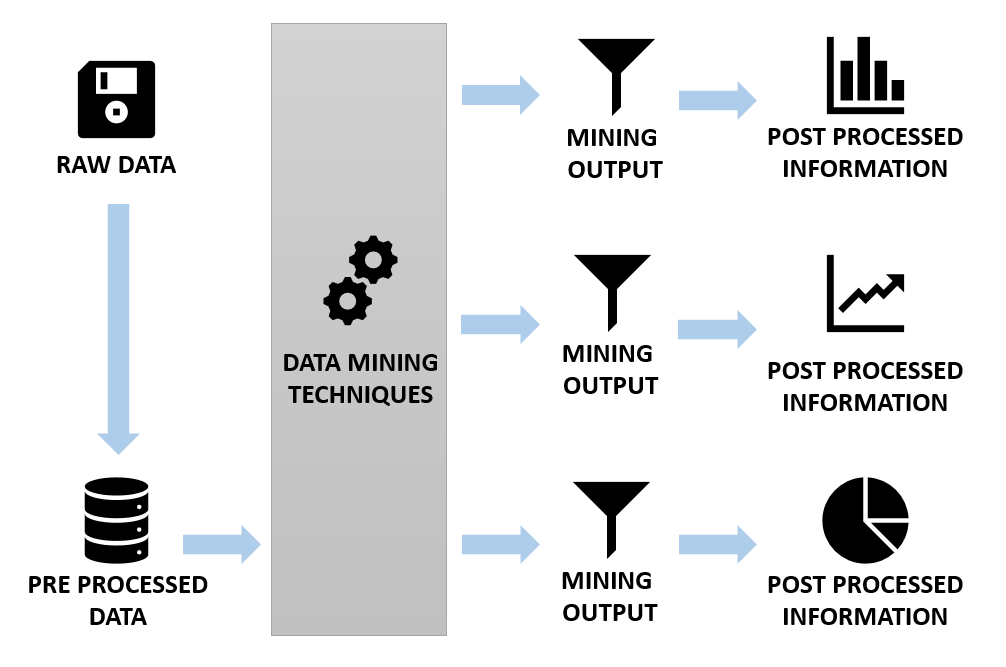
\includegraphics[scale=0.32]{img1_noback.png}
\end{centering}

\end{frame}

%-------------------------------------------------------
\begin{frame}{Introduction}{A general view about the Data Mining process}
%-------------------------------------------------------

    \centering\textit{What needs to be done?} \vspace{0,3cm}

	\begin{block}{}
		\begin{itemize}
			\item<1-> \textbf{Data Understanding}: analyze available raw data to \emph{understand} what can be extracted;
			\item<2-> \textbf{Preprocessing}: transform raw data into a \emph{minable} form, ready to be fed to the \emph{data mining algorithm};
			\item<3-> \textbf{Data Mining}: run the appropriate algorithm on the preprocessed data, to dig it for \emph{information};
			\item<4-> \textbf{Postprocessing}: display information in a human-friendly way, emphatizing what has beed dug with \emph{visualization technoques}.
		\end{itemize}
	\end{block}

\end{frame}

%-------------------------------------------------------
\begin{frame}{Introduction}{The choice of appropriate technologies}
%-------------------------------------------------------

	\centering\textit{Which technology should be employed?} \vspace{0,3cm}

	\begin{block}{}
	    \begin{itemize}
		    \item<1-> \alert{Data Processing} --- \textbf{MongoDB}: advanced \emph{dbms}, operating in the \emph{noSQL} paradigm.
		    \item<2-> \alert{Data Mining Algorithms} --- \textbf{Weka}: software which provide a \emph{framework} for running data mining algorithms.
			\item<3-> \alert{Visualization Techniques} \\
			--- \textbf{R language}: programming language with an extensive data visualization library; \\
			--- \textbf{Spreadsheets}: tabular data managing software, like Microsoft Excel and OpenOffice Calc.
	    \end{itemize}
    \end{block}

\end{frame}

\chapter{Dati Iniziali}
\label{ch:rawd}

In questo capitolo ci si soffermerà in quella che è una preliminare analisi dei dati iniziali a disposizione. Questi dati rappresentano il materiale grezzo dal quale \textit{estrarre} --- fare del \textit{mining}, come appunto il nome dell'attività suggerisce --- delle informazioni. \\

Usando come metafora una lavorazione meccanica, avere ben chiara la natura del materiale grezzo a disposizione consente di scegliere opportunamente gli utensili adatti per il lavoro da fare. Nel nostro caso, poter vantare di una comprensione generale di ciò che si ha a disposizione, potrà consentirci di scegliere le tecniche migliori per trarre il meglio dai dati iniziali. \\

\section{Carriera degli Studenti}

Una parte fondamentale dell'analisi descritta in questo lavoro è basata sul seguente data set, che contiene i dati riguardanti la produttività di tre coorti d'immatricolazione di studenti in un periodo di quattro anni. Più nel dettaglio, il dataset si compone di:

\begin{itemize}
	\item \textbf{coorte 2010}: studenti immatricolati nel 2010, carriera registrata fino agli appelli di \textbf{febbraio 2014}
	\item \textbf{coorte 2011}: studenti immatricolati nel 2011, carriera registrata fino agli appelli di \textbf{febbraio 2015}
	\item \textbf{coorte 2012}: studenti immatricolati nel 2012, carriera registrata fino agli appelli di \textbf{febbraio 2016}
	\item \textbf{coorte 2013}: studenti immatricolati nel 2013, carriera registrata fino agli appelli di \textbf{febbraio 2017}
\end{itemize}

\begin{figure}
    \centering
    \caption{Anni Accademici coperti dai dati a disposizione nel data set degli studenti}
    \label{1}
	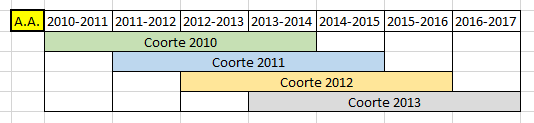
\includegraphics[scale=0.75]{../raw/stud_comp.png}
\end{figure}

Quindi, si ha a disposizione una finestra temporale di risultati ottenuti negli esami composta approssimativamente come indicato in Figura \ref{1}. Questo fatto porta ovviamente ad avere una mole d'informazioni più addensata nella parte centrale della nostra finestra temporale, avendo idealmente dati riguardanti gli esiti del maggior numero di corsi possibili solo per l'Anno Accademico 2013-2014. Tale aspetto sarà rilevante nell'interpretare i risultati di alcune analisi effettuate in seguito.

\subsection{Formato e Rappresentazione}

Il dataset è stato fornito in un unico file CSV, un formato \textit{plain text} facilmente manipolabile e interpretabile da un'ampia gamma di software. Esso si compone di una unica tabella, nella quale ogni tupla identifica uno studente, per il quale sono presenti attributi che descrivono la sua carriera universitaria nel periodo preso in esame. Oltre alle informazioni generali, quali ad esempio i risultati conseguiti nel test d'ingresso e il numero di crediti totali ottenuti nella finestra temporale esaminata, sono presenti attributi relativi alla data e al voto ottenuto in ciascun esame sostenuto. \\

Nel dettaglio, per ogni tupla rappresentante uno studente sono presenti le seguenti informazioni:

\begin{itemize}
	\item \textbf{Coorte} di immatricolazione: $$ \{2010, 2011, 2012, 2013\} $$
	\item Voto conseguito nel \textbf{test di ingresso}: $$ \{ x \in \mathbb{N} \text{ tale che } 0 \leq x \leq 25\} $$
	\item Voto ottenuto all'\textbf{esame di maturità}: $$ \{ x \in \mathbb{N} \text{ tale che } 60 \leq x \leq 100\} $$
	\item Tipo di \textbf{scuola superiore} frequentata: $$ \{LS, LC, IT, TC, IP, AL \} $$ che rappresentano rispettivamente le seguenti categorie di scuola superiore: Liceo Scientifico, Liceo Classico, Istituto Tecnico, Istituto Commerciale, Istituto Professionale, Altro
	\item \textbf{Crediti totali} ottenuti: $$ \{ x \in \mathbb{N} \text{ tale che } 0 \leq x \leq 180\} $$
	\item \textbf{Crediti} ottenuti da esami \textbf{con voto}: $$ \{ x \in \mathbb{N} \text{ tale che } 0 \leq x \leq 159\} $$
	\item \textbf{Voto medio} ottenuto negli esami: $$ \{ x \in \mathbb{N} \text{ tale che } 18 \leq x \leq 31 \text { con 31 indicante il 30 con lode}\} $$
	\item \textbf{Voto} ottenuto in un \textbf{certo esame}: $$ \{ x \in \mathbb{N} \text{ tale che } 18 \leq x \leq 31 \text { con 31 indicante il 30 con lode}\} $$
	\item \textbf{Data} in cui è stato sostenuto quell'esame: $$ \text{data in formato }MM/GG/YYYY $$
\end{itemize}

Di tutte queste informazioni, solo parte di esse sono state utilizzate in qualche analisi di \textit{data mining}, come si vedrà meglio nelle sezioni successive.

\subsection{Mole di dati}

Il dataset si compone di 208 record, ognuno dei quali ha 47 attributi. Il file che lo memorizza pesa circa 45 kb. Non si può quindi parlare propriamente di \textit{big data} in questo caso.

\section{Valutazione degli Insegnamenti}

Al fine d'integrare i dati precedenti ponendo l'attenzione sui vari corsi che compongono il Corso di Laurea, sono stati forniti i dati relativi alla valutazione dei corsi di studi da parte degli studenti. Questi dati sono ottenuti da questionari anonimi, che devono essere obbligatoriamente compilati prima di potersi prenotare per un esame. I risultati sono poi divulgati in forma aggregata, garantendo così l'anonimato dello studente. A ogni domanda lo studente ha potuto rispondere indicando un valore compreso fra zero e dieci, con zero a indicare una risposta totalmente negativa e dieci a indicare invece una risposta totalmente positiva.\\

Volendo scendere in un maggior dettaglio, sono stati forniti i dati riguardanti i seguenti anni accademici:

\begin{itemize}
	\item 2010-2011
	\item 2011-2012
	\item 2012-2013
	\item 2013-2014
	\item 2014-2015
	\item 2015-2016
	\item 2016-2017
\end{itemize}

Come si può facilmente notare, la finestra temporale coperta da questi dati va a combaciare con quella trattata dal dataset relativo alla carriera degli studenti. Questo aspetto fondamentale ha permesso di effettuare una operazione di \textit{join} fra i due dataset a disposizione, che verrà in seguito descritta nella sezione dedicata al \textit{preprocessing}.

\subsection{Formato e Rappresentazione}

Il dataset è stato fornito in sette diversi file CSV, uno per ogni anno accademico per il quale sono state espresse valutazioni dei relativi corsi. In ogni file si rappresenta una tabella le cui tuple identificano una valutazione relativa a un particolare aspetto di un corso, riportata ovviamente in forma aggregata. \\

\noindent Nel particolare, ogni record di questo tipo di tabelle è identificato dai seguenti campi, che agiscono come chiave:

\begin{itemize}
	\item \textbf{Codice identificativo}: stringa alfanumerica che identifica univocamente l'esame oggetto di valutazione all'interno del Corso di Laurea in esame.
	\item \textbf{Nome del corso}: stringa descrittiva che identifica il Corso di Laurea \textit{(in questo caso, "INFORMATICA")}.
	\item \textbf{Tipo di corso}: stringa descrittiva che identifica il tipo di Corso di Laurea \textit{(in questo caso, "Triennale")}.
	\item \textbf{Insegnamento}: stringa descrittiva che identifica l'esame oggetto di valutazione.
	\item \textbf{Docente/i}: stringa descrittiva che identifica il docente che ha tenuto il corso e svolto l'esame.
	\item \textbf{Paragrafo}: stringa descrittiva che identifica il paragrafo del questionario di valutazione.
	\item \textbf{Q}: stringa alfanumerica che identifica univocamente la domanda posta.
	\item \textbf{Quesito}: stringa descrittiva contenente il testo della domanda posta allo studente.
\end{itemize}

\noindent  Si notiche ilcampo riguardante il docente ne riporta originariamente nome e cognome per esteso. Per salvaguardarne la privacy, i valori di questo campo sono stati sostituiti con le loro immagini tramite una funzione di \textit{hash}, preservando l'unicità del valore ma nascondendo l'effettiva identità del docente. \\

A ogni tupla, identificata dai valori dei campi precedentemente descritti, corrispondono queste informazioni:

\begin{itemize}
	\item \textbf{P1, P2}: $ \{ x \in \mathbb{R} \text{ tale che } 0 \leq x \leq 100 \} $  percentuali rispettivamente di risposte sufficienti ($ \geq 6$) e insufficienti ($ < 6$).
	\item \textbf{Media}:  $ \{ x \in \mathbb{R} \text{ tale che } 0 \leq x \leq 10 \} $ media artimetica delle valutazioni ottenute.
	\item \textbf{Deviazione Standard}:  $ \{ x \in \mathbb{R} \text{ tale che } x \geq 0\} $ scarto quadratico medio delle singole valutazioni.
	\item \textbf{N}:  $ \{ x \in \mathbb{N} \text{ tale che } x \geq 6\} $ quantità di valutazioni utilizzate per calcolar ei precedenti valori.
\end{itemize}

Come è possibile intuire, molti di questi attributi sono inutili o ridondanti. Il compito di valutarne l'utilità ed eventualmente di sfoltirli sarà svolto nella fase di \textit{preprocessing}.

\subsection{Mole di dati}

I sette file forniti contengono complessivamente 2594 record, ognuno dei quali ha 13 attributi. Anche riguardo a questo dataset, non si può usare propriamente la denominazione \textit{big data}.\\

In ogni caso, visto che le quantità in gioco non sono comunque piccole, in una eventuale \textit{join} con il dataset precedente occorrerà fare particolare attenzione a non moltiplicare la quantità di record generando ridondanze, in quanto un simile errore potrebbe facilmente rendere l'insieme di dati risultante intrattabile.

\section{Conclusioni dell'Analisi dei Dati Iniziali}

Dopo aver esaminato attentamente i due dataset a disposizione, si può immediatamente affermare che il focus principale dell'analisi dovrà essere posto sui singoli corsi, per i quali si hanno molte informazioni di vario genere. \\

Volendo quindi sintetizzare quanto è stato possibile capire dall'analisi presentata in questa sezione, elaborandolo nell'ottica appena acquisita, si può riassumere la descrizione del materiale a nostra disposizione in due semplici punti:

\begin{itemize}
	\item risultati dei singoli studenti
	\item aggregazioni delle risposte ai questionari di valutazione dei corsi
\end{itemize}

Oltre a effettuare analisi sui singoli insiemi di dati, si potrà immaginare di doverli in qualche modo unire per incrociarne le informazione e trovare, possibilmente, correlazioni interessanti. Si può quindi dire che la sfida più impegnativa della prossima fase, il \textit{preprocessing}, riguardi la messa in relazione di dati aventi natura diversa. \\

Di pari passo a essa, sarà portata avanti una fase di \textit{data understanding}. Sarà utile per affinare la comprensione di quanto si è appena mostrato e per decidere il tipo di tecniche di \textit{data mining} da utilizzare sulla mole di dati a disposizione.


%-------------------------------------------------------
\section{Raw Data Understanding}
%-------------------------------------------------------
\subsection{Raw Data Sets}
\begin{frame}{Raw Data Understanding}{...}
%-------------------------------------------------------

  \begin{itemize}
	\item<1-> some item
	\item<2-> some item
	\item<3-> some other item
  \end{itemize}
\end{frame}

%-------------------------------------------------------
\section{Raw Data}
%-------------------------------------------------------
\subsection{Raw Data}
\begin{frame}{Installation}{Source files}
%-------------------------------------------------------

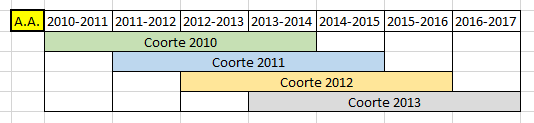
\includegraphics[scale=0.75]{../raw/stud_comp.png}


\begin{block}{}
The theme contains 4 source files:
  \begin{itemize}
	\item {\tt beamercolorthemeFeather.sty}
	\item {\tt beamerouterthemeFeather.sty}
	\item {\tt beamerinnerthemeFeather.sty}
	\item {\tt beamerthemeFeather.sty}
  \end{itemize}
\end{block}
\end{frame}

%-------------------------------------------------------
\subsection{Local and Global installation}
\begin{frame}{Installation}{Local and Global installation}
%-------------------------------------------------------
  The theme can be installed for \textbf{local} or \textbf{global} use.
  \pause
  \begin{block}{Local Installation}
  \begin{itemize}    
	\item Local installation is the simplest way of installing the theme. 
	\item You need to placing the 4 source files in the same folder as your presentation. When you download the theme, the 4 theme files are located in the {\tt local} folder.
  \end{itemize}
  \end{block}

  \begin{block}{Global Installation}
  \begin{itemize}
	 \item If you wish to make the theme globally available, you must put the files in your local latex directory tree. The location of the root of the local directory tree depends on your operating system and the latex distribution.
	 \item Detailed steps on how to proceed installation under various operating systems can be found at Beamer documentation.
  \end{itemize}
  \end{block}
\end{frame}
	 

%-------------------------------------------------------
\subsection{Required Packages}
\begin{frame}{Installation}{Required Packages}
%-------------------------------------------------------

  For using the Feather Theme you will need the Bemaer class installed and the following 2 packages
  \begin{itemize}
	\item TikZ\footnote{TikZ is a package for creating beautiful graphics. Have a look at these \chref{http://www.texample.net/tikz/examples/}{online examples} or the \chref{http://tug.ctan.org/tex-archive/graphics/pgf/base/doc/generic/pgf/pgfmanual.pdf}{pgf user manual}.}
	\item calc
  \end{itemize}
  Due to the fact that the packages are very common they should be included in your latex distribution in the first place.
\end{frame}

%-------------------------------------------------------
\section{User Interface}
\subsection{Loading the Theme and Theme Options}
\begin{frame}{User Interface}{Loading the Theme and Theme Options}
%-------------------------------------------------------

  \begin{block}{The Presentation Theme}
	The Feather Theme can be loaded in a familiar way. In the reamble of your {\tt tex} file you must type\\ \vspace{5pt} 
	{\tt \textbackslash usetheme[<options>]\{Feather\}}\\ \vspace{5pt} 
	The presentation theme loads the inner, outer and color Feather theme files and passes the {\tt <options>} on to these files.
  \end{block}
  \begin{block}{The Inner and Outher Themes}
	If you wish you can load only the inner, or the outher theme directly by\\ \vspace{5pt} 
	{\tt \textbackslash useinnertheme\{Feather\}} (and it has no options)\\ \vspace{5pt} 
	{\tt \textbackslash useoutertheme[<options>]\{Feather\}} (it has one option)\\
	\hspace{20pt}{\tt progressstyle=\{fixedCircCnt or movingCircCnt\}} \\
	\begin{itemize}
	\item which set how the progress is illustrated;
	\item the value {\tt movingCircCnt} is the default.
	\end{itemize}
  \end{block}
\end{frame}

\begin{frame}{User Interface}{Loading the Theme and Theme Options}

  \begin{block}{The Color Theme}
	Also you can load only the color theme by writing in the preamble of the {\tt tex} file 
	
	\vspace{5pt} 
	
	\begin{itemize}
	\item {\tt \textbackslash usecolortheme\{Feather\}}
	\end{itemize}
	
	\vspace{5pt}
	
	...or to change the colors of the various elements in the theme
	
	\vspace{5pt} 
	\begin{itemize}
	\item Change the bar colors: \\    
	{\tt \textbackslash setbeamercolor \{Feather\}\{fg=<color>, bg=<color>\}}
	
	\vspace{2pt} 
	
	\item Change the color of the structural elements: \\    
	{\tt \textbackslash setbeamercolor\{structure\}\{fg=<color>\}}
	
	\vspace{2pt} 
	
	\item Change the frame title text color:\\
	{\tt \textbackslash setbeamercolor\{frametitle\}\{fg=<color>\}}
	
	\vspace{2pt} 
	
	\item Change the normal text color background:    
	{\tt \textbackslash setbeamercolor\{normal text\}\{fg=<color>, bg=<color>\}}
	\end{itemize}
  \end{block}
\end{frame}


%-------------------------------------------------------
\subsection{Feather image}
\begin{frame}{User Interface}{The Feather Background Image}
%-------------------------------------------------------

\begin{block}{The Feather Background Image}
	\begin{itemize}
	\item In Feather theme, the title page frame and the last frame have the Feather image as the background image. 
	\item The Feather background image can be produced to any frame by wrating on the begining at the choosen frame the following
	\end{itemize} 
	
	\vspace{5pt} 
	
  {\tt \{\textbackslash 1bg\\
	\textbackslash begin\{frame\}[<options>]\{Frame Title\}\{Frame Subtitle\}\\
	\ldots\\
	\textbackslash end\{frame\}\}}
\end{block}
\end{frame}


{\1
\begin{frame}[plain,noframenumbering]
  \finalpage{Thank you for using Feather Beamer Theme!}
\end{frame}}

\end{document}